\begin{wrapfigure}[26]{r}[0pt]{105mm}
%	\centering
    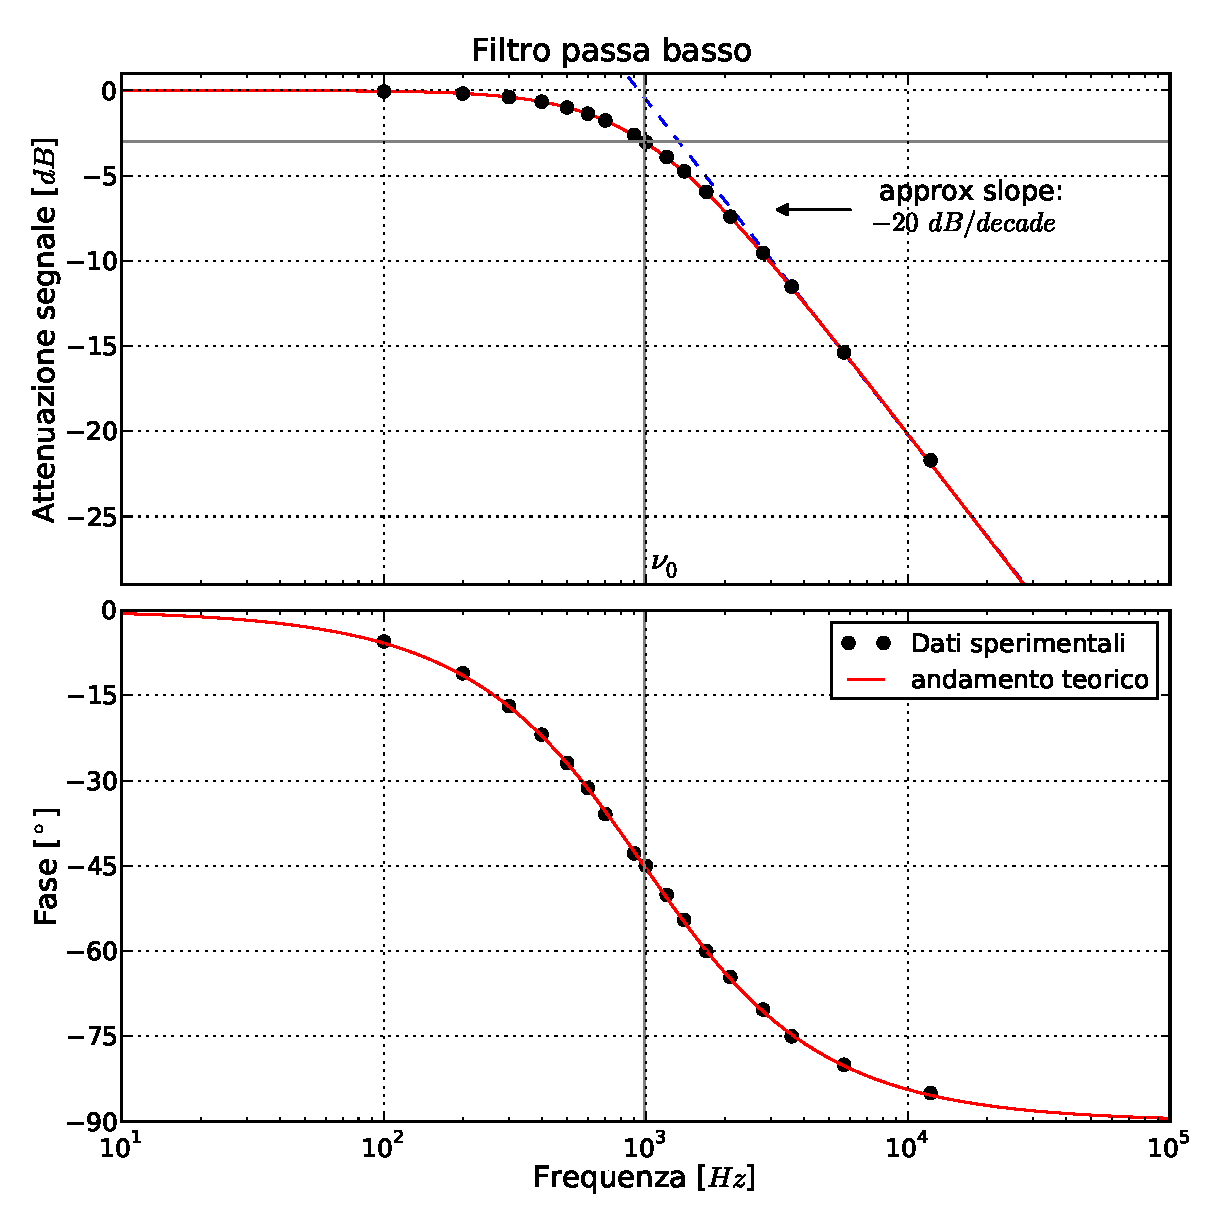
\includegraphics[width=110mm]{low.pdf}
    \caption{Diagrammi di Bode per il filtro passa basso.}
    \label{fig:low}
\end{wrapfigure}
\section{Passa basso}
Per quanto riguarda il filtro passa basso abbiamo scelto di prendere misure di tensione e differenza di fase circa ogni $5^{\circ}$, sapendo a priori che nei diagrammi di Bode l'unico valore non graficato con un logaritmo sarebbe stata la fase $\phi$.

Come mostrato in Fig.$\,$\ref{fig:circuito} a), il filtro passa basso è composto da una resistenza e da un condensatore. Intuitivamente, poichè il condensatore si comporta come un filo ideale per alte frequenze mentre come circuito aperto per le basse, si vede immediatamente che per frequenze alte i due capi dell'oscilloscopio si troveranno cortocircuitati tra loro. Dunque tale filtro farà passare le frequenze basse.

Quantitativamente, utilizzando la legge di Ohm generalizzata ($V=Z \cdot I$), ovvero introducendo il concetto di impedenze, è possibile trattare tale circuito come un partitore generalizzato. Risulta dunque semplice trovare il valore di tensione ai capi del condensatore in funzione della frequenza in input nel circuito. Una volta determinata tale funzione, è possibile calcolare il rapporto tra valore picco-picco di $V_{out}$ con $V_{in}$. \`E anche semplice ricavare la differenza di fase con il segnale in input, utilizzando la formula $\phi=arctan[\frac{Im(V_{out})}{Re(V_{out})}]$. Riportiamo le equazioni da noi calcolate analiticamente, ricordando che $Z_R=R$ e $Z_C=-\frac{j}{\omega C}$ e che $\omega\,=\,2\pi\nu$.

\noindent
\begin{minipage}{.5\linewidth}
\begin{equation}
\frac{|V_{out}|}{|V_{in}|}\,=\,\frac{1}{\sqrt{1+(RC\omega)^2}}
\label{eq:lowGain}
\end{equation}
\end{minipage}%
\begin{minipage}{.5\linewidth}
\begin{equation}
\phi=arctan(-\omega R C)
\label{eq:lowPhi}
\end{equation}
\end{minipage}\\
%\break

\noindent I valori delle componenti circuitali utilizzate sono $R=(997.81 \pm 0.01)\,\si{\ohm}$ e $C=(161 \pm 2)\,\si{\nano\farad}$.

Il diagramma di Bode\footnote{Un diagramma di Bode è una rappresentazione grafica della risposta in frequenza di un circuito e che consiste in due grafici che rappresentano rispettivamente l'ampiezza e la fase della funzione complessa di risposta in frequenza. In entrambi i grafici l'asse delle ascisse è logaritmica, mentre in quella delle ordinate vengono riportate rispettivamente il guadagno di segnale (in $\si{\decibel}$) e la fase (in gradi o radianti)} in Fig. \ref{fig:low} riporta i valori acquisiti per il filtro passa basso. Nel caso di questo filtro, si definisce una frequenza, detta di taglio, ($\nu_0=\frac{1}{2 \pi RC}\,=\,(990\pm10)\,\si{\hertz}$) tale per cui il rapporto fra l'ampiezza\footnote{la scala in decibel per la potenza è definita diversamente} dei segnali uscente ed entrante valga $\frac{|V_{out}|}{|V_{in}|}\,=\,\frac{\sqrt{2}}{2}\,=\,\frac{1}{\sqrt{2}}$. Si osserva che in questo caso il valore di guadagno vale $20Log(\frac{1}{\sqrt{2}})\,\simeq\,-3\,\si{\decibel}$ e quello di fase $\phi=-45 ^{\circ}$. Come si vede in Fig.$\,$\ref{fig:low} tale previsione teorica è confermata dai dati sperimentali.

Inoltre, nel primo diagramma, osserviamo che per valori di frequenza maggiori di quella di taglio l'attenuazione tende asintoticamente ad una retta. In base alla pendenza di tale retta, che nel nostro caso è di circa $-20\frac{\si{\decibel}}{decade}$, si definisce il \emph{fattore di bontà} del filtro passa-basso.

Notiamo infine come leggi teoriche sopra calcolate e dati sperimentali siano compatibili tra loro.
%